% \iffalse
\let\negmedspace\undefined
\let\negthickspace\undefined
\documentclass[journal,12pt,twocolumn]{IEEEtran}
\usepackage{cite}
\usepackage{amsmath,amssymb,amsfonts,amsthm}
\usepackage{algorithmic}
\usepackage{graphicx}
\usepackage{textcomp}
\usepackage{xcolor}
\usepackage{txfonts}
\usepackage{listings}
\usepackage{enumitem}
\usepackage{mathtools}
\usepackage{gensymb}
\usepackage{comment}
\usepackage[breaklinks=true]{hyperref}
\usepackage{tkz-euclide} 
\usepackage{listings}
\usepackage{gvv}                                        
\def\inputGnumericTable{}                                
\usepackage[latin1]{inputenc}                            
\usepackage{color}                                       
\usepackage{array}                                       
\usepackage{longtable}                                   
\usepackage{calc}                                        
\usepackage{multirow}                                    
\usepackage{hhline}                                      
\usepackage{ifthen}                                      
\usepackage{lscape}
\usepackage{amsmath}
\newtheorem{theorem}{Theorem}[section]
\newtheorem{problem}{Problem}
\newtheorem{proposition}{Proposition}[section]
\newtheorem{lemma}{Lemma}[section]
\newtheorem{corollary}[theorem]{Corollary}
\newtheorem{example}{Example}[section]
\newtheorem{definition}[problem]{Definition}
\newcommand{\BEQA}{\begin{eqnarray}}
\newcommand{\EEQA}{\end{eqnarray}}
\newcommand{\define}{\stackrel{\triangle}{=}}
\theoremstyle{remark}
\newtheorem{rem}{Remark}


\begin{document}

\bibliographystyle{IEEEtran}
\vspace{3cm}

\title{NCERT Mathematics Ex 9.4 Q6}
\author{EE23BTECH11059 - Tejas$^{}$% <-this % stops a space
}
\maketitle
\newpage
\textbf{Question:}
1) Find the sum to n terms of\\$3 \times 8 + 6 \times 11 + 9 \times 14 + ...$
        

    
    \solution
        
        Writing the general term of the series
        \begin{align}
            x(n)&=(3n+3)(8+3n)  
        \end{align}
        The sum of n terms of this progression can be given by:
        \begin{align}
    y\brak{n} &= x\brak{n}*u\brak{n}\\
    \implies  Y\brak{z} &= X\brak{z}U\brak{z} \label{eq:eq3}
\end{align}
$z$ transform of $x(n)$:
        \begin{align}
            X(z) &= \sum_{n=0}^{\infty} (3n+3)(3n+8)z^{-n} \\
            X(z) &= \sum_{n=0}^{\infty} (9n^2 +33n+24)z^{-n} \\
            %X(z) = 9(0(z^{-0})+1(z^{-1})+4(z)^{-2}....) + 33(0(z)^{-0} +1(z)^-%^1+2(z)^-^2....)  + 24(z^-^0+z^{-1}+z^{-2}....) 
            X(z)&=9z^{-1}\frac{(1+z^{-1})}{(1-z^{-1})^3} + \frac{33}{(1-z^{-1})^2} +24\frac{1}{1-z^{-1}}; \abs{z}>1    \label{eq:eq5}
        \end{align}
        $z$ transform of $y(n)$:\\
        using equation \eqref{eq:eq5} and equation \eqref{eq:eq3}:
        \begin{align}
         %   Y(z)&= \sum_{n=0}^{\infty} \left( \frac{33n(n+1)}{2}+\frac{9n(n+1)(2n+1)}{6} +24n) \right) \hspace{0.5cm} (6)  \\
            %Y(z)&= \frac{33}{2} \left( \sum_{n=0}^{\infty} n^2z^{-n} + \sum_{n=0}^{\infty} nz^{-n} \right) + \frac{9}{6} \left( \sum_{n=0}^{\infty} n^3z^{-n} + \sum_{n=0}^{\infty} n^2z^{-n} + \sum_{n=0}^{\infty}nz^{-n} \right) + 24\sum_{n=0}^{\infty} nz^{-n} \hspace{0.5cm} (7) \\
            Y(z)&= \frac{(18-9z^2+67)Z^{-1}}{(1-z^{-1})^3} + \frac{(42-9z^{-1})}{(1-z^{-1})^2} 
        \end{align}
        Using  \eqref{eq:1/ap/contour} to find the inverse Z-transform,
        %\begin{align}
         %   R & =\frac{1}{(m-1) !} \lim _{z \rightarrow a} \frac{d^{m-1}}{d z^{m-1}}\brak{(z-a)^m f(z)}
        %\end{align}
        
        We get $y(n)$ as: 
        \begin{align}
            y(n)=\frac{33n(n+1)}{2}+\frac{9n(n+1)(2 n+1)}{6}+24n
        \end{align}
        
        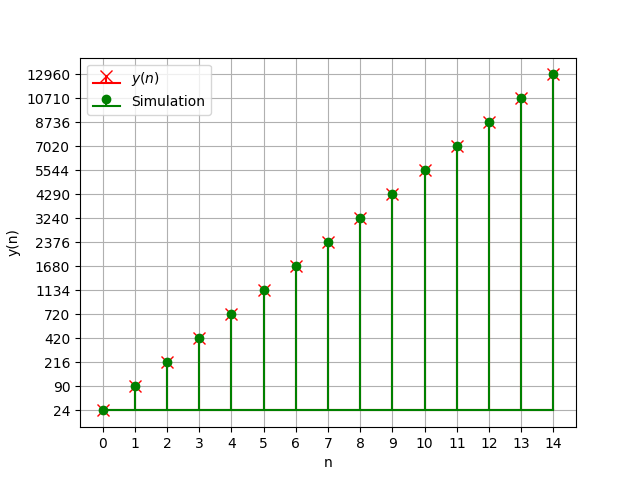
\includegraphics[width=\columnwidth]{figs/plot.png}

        
            
           
             
             
             
        

        













\renewcommand{\thefigure}{\theenumi}
\renewcommand{\thetable}{\theenumi}






